\documentclass[tikz,border=0pt]{standalone}
\usepackage{lmodern}
\usetikzlibrary{arrows.meta}
\definecolor{badge}{HTML}{2CA02C}
\begin{document}
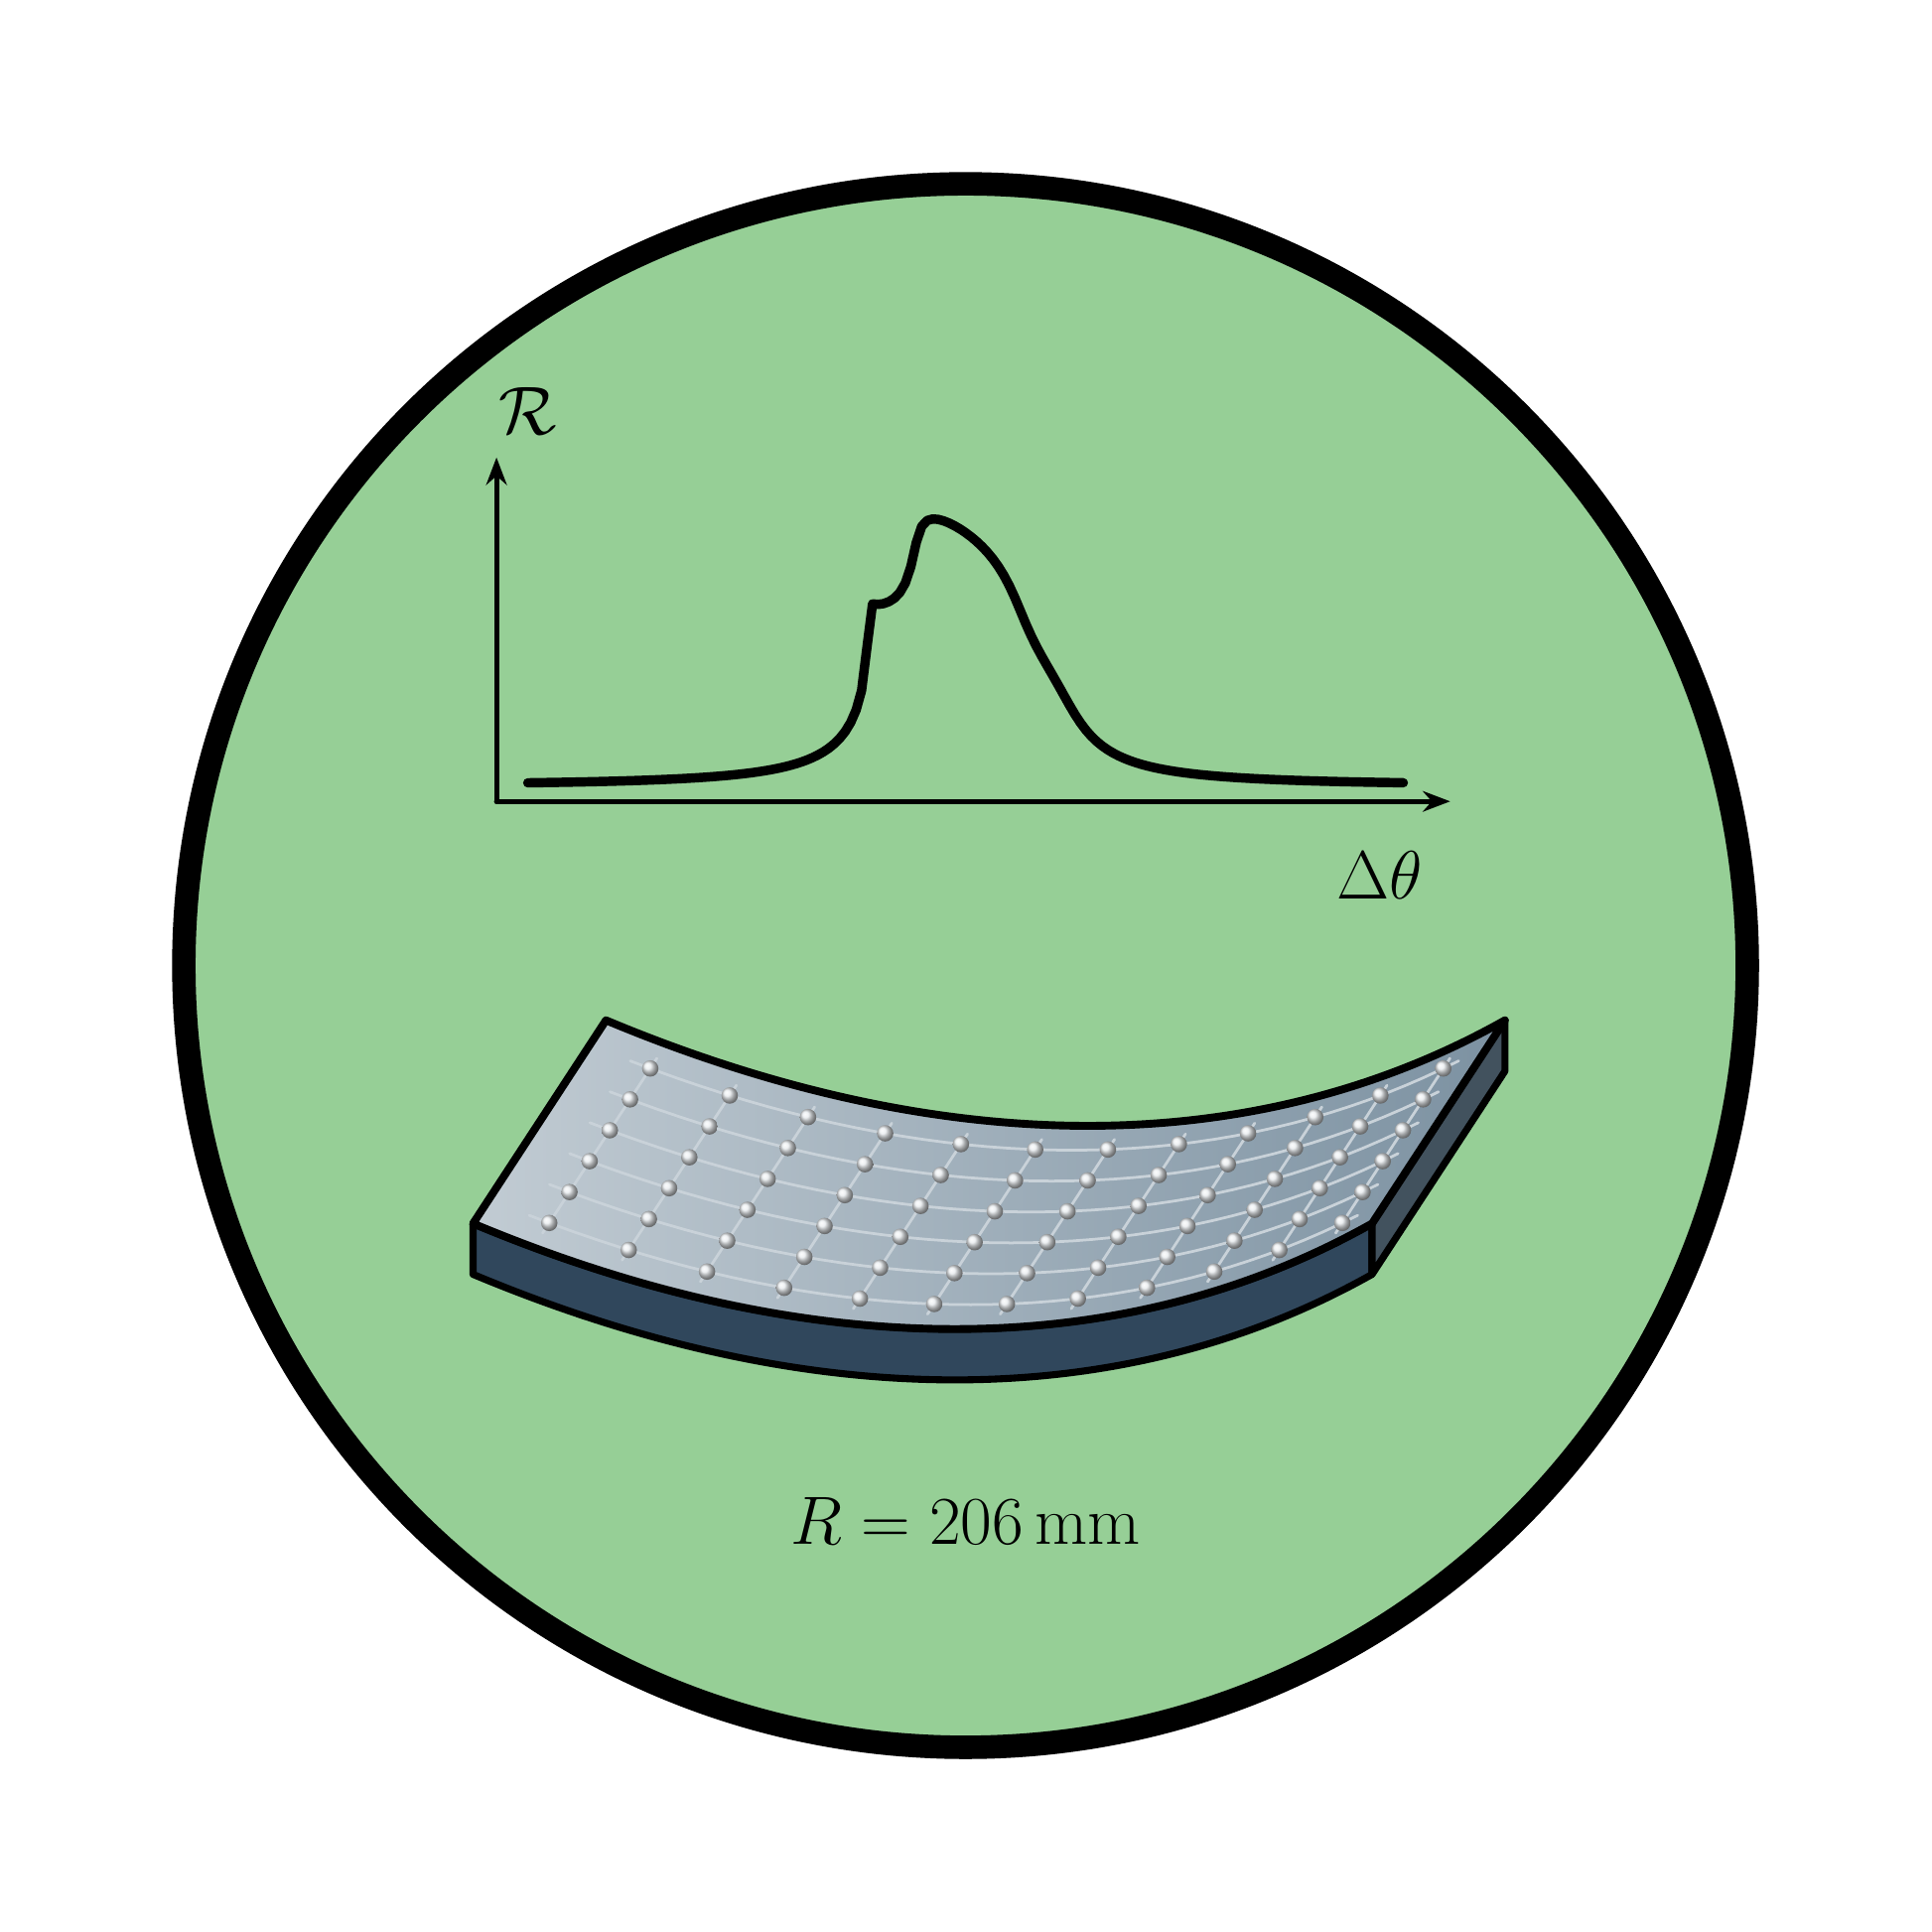
\begin{tikzpicture}[x=10mm,y=10mm,line cap=round,line join=round]
\path[use as bounding box] (-12,-12) rectangle (12,12);
\filldraw[fill=badge!50!white,draw=black,line width=3mm] (0,0) circle (10);

% Curve: flat perfect Ge(880), 25.5 keV, 1 mm, unpolarized.
% Calculated using 2_Lower_Reflection/s1_reflection.py (crystalpy).
% Illustration below: bent crystal; curve does not include bending/strain.
\draw[black,line width=.65mm,-{Stealth[length=3.5mm]}] (-6,2.1) -- (6.2,2.1);
\draw[black,line width=.65mm,-{Stealth[length=3.5mm]}] (-6,2.1) -- (-6,6.5);
\node[font=\fontsize{32}{36}\selectfont] at (-5.6,7.1) {$\mathcal{R}$};
\node[font=\fontsize{30}{34}\selectfont] at (5.3,1.15) {$\Delta\theta$};
\draw[black,line width=1.2mm] plot coordinates {(-5.6000,2.3374) (-5.5300,2.3384) (-5.4600,2.3394) (-5.3900,2.3405) (-5.3200,2.3415) (-5.2500,2.3427) (-5.1800,2.3439) (-5.1100,2.3451) (-5.0400,2.3464) (-4.9700,2.3477) (-4.9000,2.3491) (-4.8300,2.3506) (-4.7600,2.3521) (-4.6900,2.3537) (-4.6200,2.3554) (-4.5500,2.3572) (-4.4800,2.3590) (-4.4100,2.3610) (-4.3400,2.3630) (-4.2700,2.3652) (-4.2000,2.3674) (-4.1300,2.3698) (-4.0600,2.3723) (-3.9900,2.3750) (-3.9200,2.3778) (-3.8500,2.3807) (-3.7800,2.3839) (-3.7100,2.3872) (-3.6400,2.3907) (-3.5700,2.3945) (-3.5000,2.3985) (-3.4300,2.4028) (-3.3600,2.4074) (-3.2900,2.4122) (-3.2200,2.4175) (-3.1500,2.4231) (-3.0800,2.4291) (-3.0100,2.4356) (-2.9400,2.4427) (-2.8700,2.4503) (-2.8000,2.4586) (-2.7300,2.4675) (-2.6600,2.4774) (-2.5900,2.4881) (-2.5200,2.4999) (-2.4500,2.5129) (-2.3800,2.5273) (-2.3100,2.5432) (-2.2400,2.5611) (-2.1700,2.5811) (-2.1000,2.6037) (-2.0300,2.6294) (-1.9600,2.6589) (-1.8900,2.6930) (-1.8200,2.7327) (-1.7500,2.7798) (-1.6800,2.8365) (-1.6100,2.9060) (-1.5400,2.9936) (-1.4700,3.1085) (-1.4000,3.2685) (-1.3300,3.5186) (-1.2600,4.0816) (-1.1900,4.6270) (-1.1200,4.6199) (-1.0500,4.6297) (-0.9800,4.6549) (-0.9100,4.6995) (-0.8400,4.7728) (-0.7700,4.8940) (-0.7000,5.1023) (-0.6300,5.4125) (-0.5600,5.6197) (-0.4900,5.6934) (-0.4200,5.7127) (-0.3500,5.7074) (-0.2800,5.6883) (-0.2100,5.6602) (-0.1400,5.6251) (-0.0700,5.5842) (0.0000,5.5376) (0.0700,5.4852) (0.1400,5.4265) (0.2100,5.3606) (0.2800,5.2862) (0.3500,5.2014) (0.4200,5.1039) (0.4900,4.9906) (0.5600,4.8586) (0.6300,4.7069) (0.7000,4.5408) (0.7700,4.3731) (0.8400,4.2166) (0.9100,4.0752) (0.9800,3.9460) (1.0500,3.8234) (1.1200,3.7024) (1.1900,3.5795) (1.2600,3.4542) (1.3300,3.3296) (1.4000,3.2113) (1.4700,3.1045) (1.5400,3.0116) (1.6100,2.9322) (1.6800,2.8650) (1.7500,2.8079) (1.8200,2.7593) (1.8900,2.7175) (1.9600,2.6813) (2.0300,2.6499) (2.1000,2.6223) (2.1700,2.5980) (2.2400,2.5765) (2.3100,2.5573) (2.3800,2.5401) (2.4500,2.5246) (2.5200,2.5107) (2.5900,2.4980) (2.6600,2.4865) (2.7300,2.4759) (2.8000,2.4663) (2.8700,2.4575) (2.9400,2.4493) (3.0100,2.4418) (3.0800,2.4349) (3.1500,2.4285) (3.2200,2.4225) (3.2900,2.4169) (3.3600,2.4118) (3.4300,2.4069) (3.5000,2.4024) (3.5700,2.3982) (3.6400,2.3942) (3.7100,2.3905) (3.7800,2.3869) (3.8500,2.3836) (3.9200,2.3805) (3.9900,2.3776) (4.0600,2.3748) (4.1300,2.3721) (4.2000,2.3696) (4.2700,2.3673) (4.3400,2.3650) (4.4100,2.3629) (4.4800,2.3609) (4.5500,2.3589) (4.6200,2.3571) (4.6900,2.3553) (4.7600,2.3536) (4.8300,2.3520) (4.9000,2.3505) (4.9700,2.3491) (5.0400,2.3477) (5.1100,2.3463) (5.1800,2.3450) (5.2500,2.3438) (5.3200,2.3426) (5.3900,2.3415) (5.4600,2.3404) (5.5300,2.3394) (5.6000,2.3383)};

\definecolor{wafer}{HTML}{657E91}
\definecolor{edge}{HTML}{30475C}
\begin{scope}[yshift=-33mm]
\path[fill=edge,draw=black,line width=.9mm]
 (-6.3,0) .. controls (-2,-1.8) and (2,-1.8) .. (5.2,0)
 -- (5.2,-.65) .. controls (2,-2.45) and (-2,-2.45) .. (-6.3,-.65) -- cycle;
\path[fill=wafer!65!black,draw=black,line width=.9mm]
 (5.2,0) -- (6.9,2.6) -- (6.9,1.95) -- (5.2,-.65) -- cycle;
\path[shade,left color=wafer!40!white,right color=wafer!85!white,draw=black,line width=1mm]
 (-6.3,0) .. controls (-2,-1.8) and (2,-1.8) .. (5.2,0)
 -- (6.9,2.6) .. controls (3.7,.8) and (-.3,.8) .. (-4.6,2.6) -- cycle;
\draw[white!65!wafer,line width=.35mm] plot coordinates {(-5.5815,0.1046) (-5.2870,-0.0068) (-4.9936,-0.1125) (-4.7012,-0.2124) (-4.4100,-0.3067) (-4.1200,-0.3953) (-3.8311,-0.4781) (-3.5435,-0.5552) (-3.2572,-0.6266) (-2.9721,-0.6924) (-2.6885,-0.7523) (-2.4061,-0.8066) (-2.1252,-0.8552) (-1.8458,-0.8980) (-1.5679,-0.9352) (-1.2914,-0.9666) (-1.0166,-0.9923) (-0.7433,-1.0123) (-0.4717,-1.0266) (-0.2017,-1.0351) (0.0665,-1.0380) (0.3330,-1.0351) (0.5977,-1.0266) (0.8606,-1.0123) (1.1216,-0.9923) (1.3808,-0.9666) (1.6380,-0.9352) (1.8933,-0.8980) (2.1465,-0.8552) (2.3977,-0.8066) (2.6469,-0.7523) (2.8939,-0.6924) (3.1388,-0.6266) (3.3815,-0.5552) (3.6220,-0.4781) (3.8602,-0.3953) (4.0961,-0.3067) (4.3297,-0.2124) (4.5610,-0.1125) (4.7898,-0.0068) (5.0162,0.1046)};
\draw[white!65!wafer,line width=.35mm] plot coordinates {(-5.3231,0.4998) (-5.0286,0.3884) (-4.7352,0.2827) (-4.4428,0.1828) (-4.1516,0.0885) (-3.8616,-0.0001) (-3.5727,-0.0829) (-3.2851,-0.1600) (-2.9988,-0.2314) (-2.7137,-0.2972) (-2.4301,-0.3571) (-2.1477,-0.4114) (-1.8668,-0.4600) (-1.5874,-0.5028) (-1.3095,-0.5400) (-1.0330,-0.5714) (-0.7582,-0.5971) (-0.4849,-0.6171) (-0.2133,-0.6314) (0.0567,-0.6399) (0.3249,-0.6428) (0.5914,-0.6399) (0.8561,-0.6314) (1.1190,-0.6171) (1.3800,-0.5971) (1.6392,-0.5714) (1.8964,-0.5400) (2.1517,-0.5028) (2.4049,-0.4600) (2.6561,-0.4114) (2.9053,-0.3571) (3.1523,-0.2972) (3.3972,-0.2314) (3.6399,-0.1600) (3.8804,-0.0829) (4.1186,-0.0001) (4.3545,0.0885) (4.5881,0.1828) (4.8194,0.2827) (5.0482,0.3884) (5.2746,0.4998)};
\draw[white!65!wafer,line width=.35mm] plot coordinates {(-5.0647,0.8950) (-4.7702,0.7836) (-4.4768,0.6779) (-4.1844,0.5780) (-3.8932,0.4837) (-3.6032,0.3951) (-3.3143,0.3123) (-3.0267,0.2352) (-2.7404,0.1638) (-2.4553,0.0980) (-2.1717,0.0381) (-1.8893,-0.0162) (-1.6084,-0.0648) (-1.3290,-0.1076) (-1.0511,-0.1448) (-0.7746,-0.1762) (-0.4998,-0.2019) (-0.2265,-0.2219) (0.0451,-0.2362) (0.3151,-0.2447) (0.5833,-0.2476) (0.8498,-0.2447) (1.1145,-0.2362) (1.3774,-0.2219) (1.6384,-0.2019) (1.8976,-0.1762) (2.1548,-0.1448) (2.4101,-0.1076) (2.6633,-0.0648) (2.9145,-0.0162) (3.1637,0.0381) (3.4107,0.0980) (3.6556,0.1638) (3.8983,0.2352) (4.1388,0.3123) (4.3770,0.3951) (4.6129,0.4837) (4.8465,0.5780) (5.0778,0.6779) (5.3066,0.7836) (5.5330,0.8950)};
\draw[white!65!wafer,line width=.35mm] plot coordinates {(-4.8063,1.2902) (-4.5118,1.1788) (-4.2184,1.0731) (-3.9260,0.9732) (-3.6348,0.8789) (-3.3448,0.7903) (-3.0559,0.7075) (-2.7683,0.6304) (-2.4820,0.5590) (-2.1969,0.4932) (-1.9133,0.4333) (-1.6309,0.3790) (-1.3500,0.3304) (-1.0706,0.2876) (-0.7927,0.2504) (-0.5162,0.2190) (-0.2414,0.1933) (0.0319,0.1733) (0.3035,0.1590) (0.5735,0.1505) (0.8417,0.1476) (1.1082,0.1505) (1.3729,0.1590) (1.6358,0.1733) (1.8968,0.1933) (2.1560,0.2190) (2.4132,0.2504) (2.6685,0.2876) (2.9217,0.3304) (3.1729,0.3790) (3.4221,0.4333) (3.6691,0.4932) (3.9140,0.5590) (4.1567,0.6304) (4.3972,0.7075) (4.6354,0.7903) (4.8713,0.8789) (5.1049,0.9732) (5.3362,1.0731) (5.5650,1.1788) (5.7914,1.2902)};
\draw[white!65!wafer,line width=.35mm] plot coordinates {(-4.5479,1.6854) (-4.2534,1.5740) (-3.9600,1.4683) (-3.6676,1.3684) (-3.3764,1.2741) (-3.0864,1.1855) (-2.7975,1.1027) (-2.5099,1.0256) (-2.2236,0.9542) (-1.9385,0.8884) (-1.6549,0.8285) (-1.3725,0.7742) (-1.0916,0.7256) (-0.8122,0.6828) (-0.5343,0.6456) (-0.2578,0.6142) (0.0170,0.5885) (0.2903,0.5685) (0.5619,0.5542) (0.8319,0.5457) (1.1001,0.5428) (1.3666,0.5457) (1.6313,0.5542) (1.8942,0.5685) (2.1552,0.5885) (2.4144,0.6142) (2.6716,0.6456) (2.9269,0.6828) (3.1801,0.7256) (3.4313,0.7742) (3.6805,0.8285) (3.9275,0.8884) (4.1724,0.9542) (4.4151,1.0256) (4.6556,1.1027) (4.8938,1.1855) (5.1297,1.2741) (5.3633,1.3684) (5.5946,1.4683) (5.8234,1.5740) (6.0498,1.6854)};
\draw[white!65!wafer,line width=.35mm] plot coordinates {(-4.2895,2.0806) (-3.9950,1.9692) (-3.7016,1.8635) (-3.4092,1.7636) (-3.1180,1.6693) (-2.8280,1.5807) (-2.5391,1.4979) (-2.2515,1.4208) (-1.9652,1.3494) (-1.6801,1.2836) (-1.3965,1.2237) (-1.1141,1.1694) (-0.8332,1.1208) (-0.5538,1.0780) (-0.2759,1.0408) (0.0006,1.0094) (0.2754,0.9837) (0.5487,0.9637) (0.8203,0.9494) (1.0903,0.9409) (1.3585,0.9380) (1.6250,0.9409) (1.8897,0.9494) (2.1526,0.9637) (2.4136,0.9837) (2.6728,1.0094) (2.9300,1.0408) (3.1853,1.0780) (3.4385,1.1208) (3.6897,1.1694) (3.9389,1.2237) (4.1859,1.2836) (4.4308,1.3494) (4.6735,1.4208) (4.9140,1.4979) (5.1522,1.5807) (5.3881,1.6693) (5.6217,1.7636) (5.8530,1.8635) (6.0818,1.9692) (6.3082,2.0806)};
\draw[white!65!wafer,line width=.35mm] (-5.4103,-0.1226) -- (-3.9483,2.1134);
\draw[white!65!wafer,line width=.35mm] (-4.3940,-0.4682) -- (-2.9320,1.7678);
\draw[white!65!wafer,line width=.35mm] (-3.3919,-0.7446) -- (-1.9299,1.4914);
\draw[white!65!wafer,line width=.35mm] (-2.4055,-0.9520) -- (-0.9435,1.2840);
\draw[white!65!wafer,line width=.35mm] (-1.4364,-1.0902) -- (0.0256,1.1458);
\draw[white!65!wafer,line width=.35mm] (-0.4861,-1.1594) -- (0.9759,1.0766);
\draw[white!65!wafer,line width=.35mm] (0.4438,-1.1594) -- (1.9058,1.0766);
\draw[white!65!wafer,line width=.35mm] (1.3519,-1.0902) -- (2.8139,1.1458);
\draw[white!65!wafer,line width=.35mm] (2.2365,-0.9520) -- (3.6985,1.2840);
\draw[white!65!wafer,line width=.35mm] (3.0962,-0.7446) -- (4.5582,1.4914);
\draw[white!65!wafer,line width=.35mm] (3.9293,-0.4682) -- (5.3913,1.7678);
\draw[white!65!wafer,line width=.35mm] (4.7345,-0.1226) -- (6.1965,2.1134);
\shade[ball color=white!85!wafer] (-4.0333,1.9834) circle (.105);
\shade[ball color=white!85!wafer] (-3.0170,1.6378) circle (.105);
\shade[ball color=white!85!wafer] (-2.0149,1.3614) circle (.105);
\shade[ball color=white!85!wafer] (-1.0285,1.1540) circle (.105);
\shade[ball color=white!85!wafer] (-0.0594,1.0158) circle (.105);
\shade[ball color=white!85!wafer] (0.8909,0.9466) circle (.105);
\shade[ball color=white!85!wafer] (1.8208,0.9466) circle (.105);
\shade[ball color=white!85!wafer] (2.7289,1.0158) circle (.105);
\shade[ball color=white!85!wafer] (3.6135,1.1540) circle (.105);
\shade[ball color=white!85!wafer] (4.4732,1.3614) circle (.105);
\shade[ball color=white!85!wafer] (5.3063,1.6378) circle (.105);
\shade[ball color=white!85!wafer] (6.1115,1.9834) circle (.105);
\shade[ball color=white!85!wafer] (-4.2917,1.5882) circle (.105);
\shade[ball color=white!85!wafer] (-3.2754,1.2426) circle (.105);
\shade[ball color=white!85!wafer] (-2.2733,0.9662) circle (.105);
\shade[ball color=white!85!wafer] (-1.2869,0.7588) circle (.105);
\shade[ball color=white!85!wafer] (-0.3178,0.6206) circle (.105);
\shade[ball color=white!85!wafer] (0.6325,0.5514) circle (.105);
\shade[ball color=white!85!wafer] (1.5624,0.5514) circle (.105);
\shade[ball color=white!85!wafer] (2.4705,0.6206) circle (.105);
\shade[ball color=white!85!wafer] (3.3551,0.7588) circle (.105);
\shade[ball color=white!85!wafer] (4.2148,0.9662) circle (.105);
\shade[ball color=white!85!wafer] (5.0479,1.2426) circle (.105);
\shade[ball color=white!85!wafer] (5.8531,1.5882) circle (.105);
\shade[ball color=white!85!wafer] (-4.5501,1.1930) circle (.105);
\shade[ball color=white!85!wafer] (-3.5338,0.8474) circle (.105);
\shade[ball color=white!85!wafer] (-2.5317,0.5710) circle (.105);
\shade[ball color=white!85!wafer] (-1.5453,0.3636) circle (.105);
\shade[ball color=white!85!wafer] (-0.5762,0.2254) circle (.105);
\shade[ball color=white!85!wafer] (0.3741,0.1562) circle (.105);
\shade[ball color=white!85!wafer] (1.3040,0.1562) circle (.105);
\shade[ball color=white!85!wafer] (2.2121,0.2254) circle (.105);
\shade[ball color=white!85!wafer] (3.0967,0.3636) circle (.105);
\shade[ball color=white!85!wafer] (3.9564,0.5710) circle (.105);
\shade[ball color=white!85!wafer] (4.7895,0.8474) circle (.105);
\shade[ball color=white!85!wafer] (5.5947,1.1930) circle (.105);
\shade[ball color=white!85!wafer] (-4.8085,0.7978) circle (.105);
\shade[ball color=white!85!wafer] (-3.7922,0.4522) circle (.105);
\shade[ball color=white!85!wafer] (-2.7901,0.1758) circle (.105);
\shade[ball color=white!85!wafer] (-1.8037,-0.0316) circle (.105);
\shade[ball color=white!85!wafer] (-0.8346,-0.1698) circle (.105);
\shade[ball color=white!85!wafer] (0.1157,-0.2390) circle (.105);
\shade[ball color=white!85!wafer] (1.0456,-0.2390) circle (.105);
\shade[ball color=white!85!wafer] (1.9537,-0.1698) circle (.105);
\shade[ball color=white!85!wafer] (2.8383,-0.0316) circle (.105);
\shade[ball color=white!85!wafer] (3.6980,0.1758) circle (.105);
\shade[ball color=white!85!wafer] (4.5311,0.4522) circle (.105);
\shade[ball color=white!85!wafer] (5.3363,0.7978) circle (.105);
\shade[ball color=white!85!wafer] (-5.0669,0.4026) circle (.105);
\shade[ball color=white!85!wafer] (-4.0506,0.0570) circle (.105);
\shade[ball color=white!85!wafer] (-3.0485,-0.2194) circle (.105);
\shade[ball color=white!85!wafer] (-2.0621,-0.4268) circle (.105);
\shade[ball color=white!85!wafer] (-1.0930,-0.5650) circle (.105);
\shade[ball color=white!85!wafer] (-0.1427,-0.6342) circle (.105);
\shade[ball color=white!85!wafer] (0.7872,-0.6342) circle (.105);
\shade[ball color=white!85!wafer] (1.6953,-0.5650) circle (.105);
\shade[ball color=white!85!wafer] (2.5799,-0.4268) circle (.105);
\shade[ball color=white!85!wafer] (3.4396,-0.2194) circle (.105);
\shade[ball color=white!85!wafer] (4.2727,0.0570) circle (.105);
\shade[ball color=white!85!wafer] (5.0779,0.4026) circle (.105);
\shade[ball color=white!85!wafer] (-5.3253,0.0074) circle (.105);
\shade[ball color=white!85!wafer] (-4.3090,-0.3382) circle (.105);
\shade[ball color=white!85!wafer] (-3.3069,-0.6146) circle (.105);
\shade[ball color=white!85!wafer] (-2.3205,-0.8220) circle (.105);
\shade[ball color=white!85!wafer] (-1.3514,-0.9602) circle (.105);
\shade[ball color=white!85!wafer] (-0.4011,-1.0294) circle (.105);
\shade[ball color=white!85!wafer] (0.5288,-1.0294) circle (.105);
\shade[ball color=white!85!wafer] (1.4369,-0.9602) circle (.105);
\shade[ball color=white!85!wafer] (2.3215,-0.8220) circle (.105);
\shade[ball color=white!85!wafer] (3.1812,-0.6146) circle (.105);
\shade[ball color=white!85!wafer] (4.0143,-0.3382) circle (.105);
\shade[ball color=white!85!wafer] (4.8195,0.0074) circle (.105);
\end{scope}
\node[font=\fontsize{30}{36}\selectfont] at (0,-7.1) {$R=206\,\mathrm{mm}$};
\end{tikzpicture}
\end{document}
